% This is LLNCS.DEM the demonstration file of
% the LaTeX macro package from Springer-Verlag
% for Lecture Notes in Computer Science,
% version 2.4 for LaTeX2e as of 16. April 2010
%
\documentclass{llncs}
%
\usepackage{amsmath}
\usepackage{amssymb}
\usepackage{tikz}

\newcounter{instr}
\newcommand{\ninstr}{\refstepcounter{instr}\theinstr.}

\begin{document}

\title{Species delimitation}

\titlerunning{Species delimitation}

\author{Tom\'{a}\v{s} Flouri1\inst{1} \and Paschalia Kapli\inst{1} \and Sarah Lutteropp\inst{1}}
\authorrunning{Tom\'{a}\v{s} Flouri et al.} % abbreviated author list
\institute{Heidelberg Institute of Theoretical Studies}

\maketitle

\begin{abstract}
An explanation of the single-lambda and multiple-lambda heuristic for PTP.
\end{abstract}

\section{Related Work}

The heuristic works similar to the algorithm from Gulek et al.\cite{Gulek:2010:DPA:1838770.1839019}.

\ldots

\section{Task Description}

Given a rooted fully binary tree with edge weight function $w$, we want to partition its leaves into disjoint sets (called species). The MRCAs of those species induce subtrees $A_1, \ldots, A_{k}$. Every edge that is not assigned to one of these subtrees is then put into the set of speciation edges, $A_{k+1}$.

\paragraph{Multiple Lambda Score}

We want to find a delimitation such that the following sum of loglikelihoods (in the following referred to as \emph{score}) is maximized:

$$\sum_{i=1}^{k+1}{ \left(|A_i| * \log |A_i| - |A_i| - |A_i| * \log\left( \sum_{e \in A_i}{w(e)} \right) \right)}$$

\paragraph{Single Lambda Score}

We want to find a delimitation such that the following sum of loglikelihoods (in the following referred to as \emph{score}, too) is maximized:

$$\left(\sum_{i=1}^{k}{|A_i|} * \log\left(\sum_{i=1}^{k}{|A_i|}\right) - \sum_{i=1}^{k}{|A_i|} - \sum_{i=1}^{k}{|A_i|} * \log \left( \sum_{e \in A_i \cup \ldots \cup A_k}{w(e)} \right)\right)$$

$$ + \left(|A_{k+1}| * \log |A_{k+1}| - |A_{k+1}| - |A_{k+1}| * \log\left( \sum_{e \in A_{k+1}}{w(e)} \right) \right)$$

\section{General Idea}

We follow a bottom-up dynamic programming approach, always trying to extend a good solution for the children subtrees in order to obtain a good solution for the currently observed tree.

\subsection{Currently observed tree}

For each node $v$, the \emph{currently observed tree} consists of the subtree rooted at $v$, $S(v)$, and the set of edges where we already know that they have to be speciation edges in the case that $S(v)$ contains any speciation edges. (see Fig.~\ref{fig:currently_observed_tree})

\begin{figure}[h!]
	\centering
	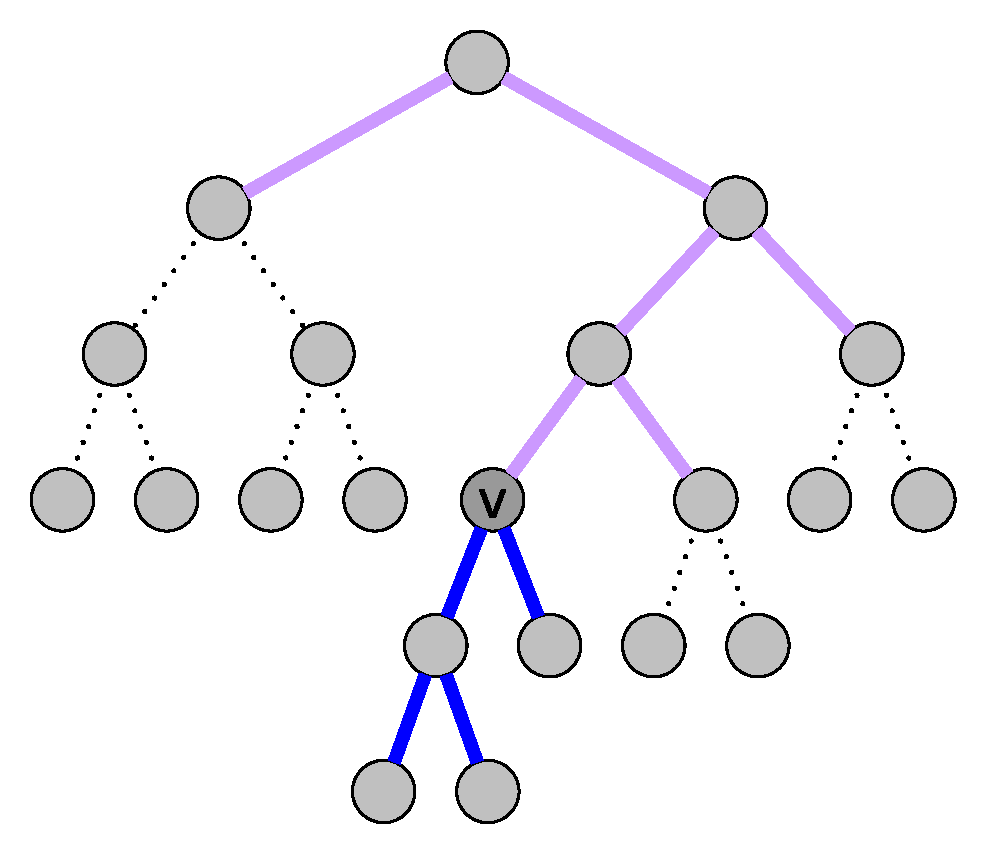
\includegraphics[scale=0.4]{images/currently_observed_tree.pdf}
	\caption{The currently observed tree of $v$, marked with thick blue edges}
	\label{fig:currently_observed_tree}
\end{figure}

For every node, we store an array that contains the best found score for $0, 2, 4, \ldots$ speciation edges.

In order to determine a good solution for $v$ that contains $k+2$ speciation edges, we combine all solutions for $i$ speciation edges from the left child of $v$ with all solutions for $j$ speciation edges for the right child of $v$ where $i+j=k$ and take the one that yields to the highest score. (TODO: Image)

If we have $0$ speciation edges in $S(v)$, it simply means that $v$ is handled as the root of a coalescent group (species). Thus we can directly use the score function to obtain this score and do not need to look at the children's scores.

\ldots

\section{Handling of zero-length Edges}

\ldots

\bibliographystyle{splncs03}
\bibliography{delimit}
\end{document}
